\documentclass[a4paper,11pt, twocolumn]{article}
\usepackage[margin=0.8in]{geometry}
\usepackage{xcolor}
\usepackage{graphicx} %package to manage images
\graphicspath{ {./images/} }
\usepackage{float}
\usepackage{tabularx}
\usepackage{multirow}
\usepackage[fleqn]{mathtools}

\title{AS-1 Combinational Logic}
\author{Revision sheet}
\date{}

\usepackage{fancyhdr}
\pagestyle{fancy}
\fancyhead{} % clear all header fields
\renewcommand{\headrulewidth}{0pt} % no line in header area
\fancyfoot{} % clear all footer fields
\renewcommand{\footrulewidth}{0.4pt}
\fancyfoot[C]{\thepage} % page number in centre of the page
\fancyfoot[R]{\footnotesize Thomas Boxall \\ Images from WJEC E-Book} % right hand footer has author name on top line and images reference on bottom line
\fancyfoot[L]{\footnotesize AS-1 Combinational Logic \\ Revision sheet} % left hand footer has title of document on top line and 'Revision Sheet' on bottom line


\begin{document}

\maketitle
\thispagestyle{fancy}

% CONTENTS OF THE REVISION SHEET HERE

\section{Signals}
There are two types of signals.
\subsection{Analogue Signal}
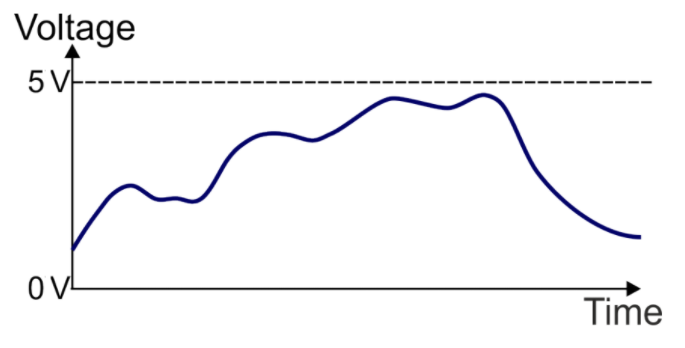
\includegraphics[width=0.4\textwidth]{analogueGraph.PNG}\\
Analogue signals can have any value between the minimum and maximum.
\subsection{Digital Signals}
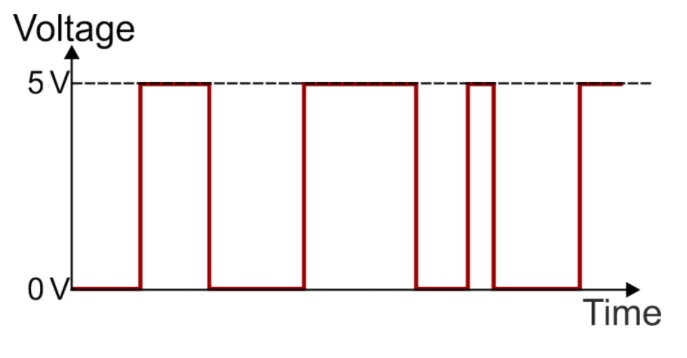
\includegraphics[width=0.4\textwidth]{digitalGraph.PNG}\\
Digital signals can either be on (logic 1 / +5V) or off (logic 0 / 0V).

\section{Digital Inputs and Outputs}
There are a number of different digital input components: Push-To-Make button; Push-To-Break button; latching switch. 
\subsection{Push-To-Make Buttons}
Buttons require a pull up or pull down resistor. This will make sure that when the button isn't pressed (in the case of PTM), the value outputted is an actual value, not undefined/floating.
\subsubsection{Active High button}
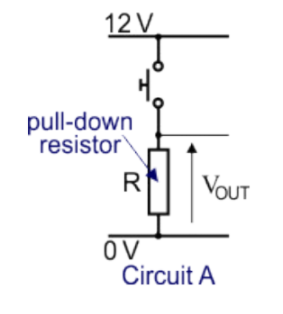
\includegraphics[width=0.4\textwidth]{activeHighButton.PNG}\\
This is normally outputting a low signal until the button is pressed, then it outputs a high signal.
\subsubsection{Active Low Button}
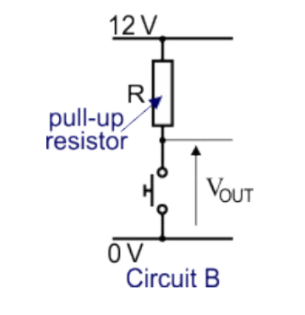
\includegraphics[width=0.4\textwidth]{activeLowButton.PNG}\\
This is normally outputting a high signal until the button is pressed, then it outputs a low signal.
\subsection{Sourcing and Sinking}
Logic gates can either source or sink current. This means they can either output current or take in current. This is extremely useful as it allows us to power active high and active low components off of the outputs of logic gates.
\subsubsection{Sourcing}
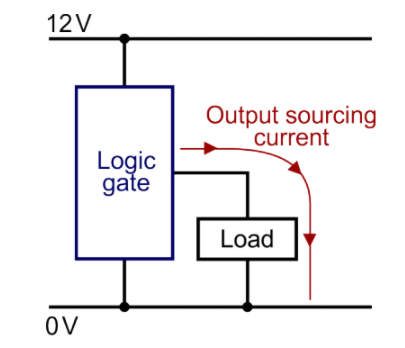
\includegraphics[width=0.4\textwidth]{sourcing.PNG}\\
Current flows from the gate to the 0V rail. The gate is sourcing current.
\subsubsection{Sinking}
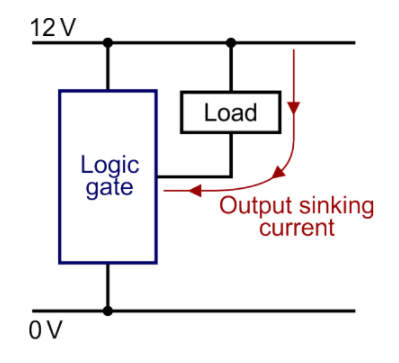
\includegraphics[width=0.4\textwidth]{sinking.PNG}\\
Current flows from the load and into the gate. The gate is sinking current.

\section{Logic Gates and Truth Tables}
For the most part, logic gates can have multiple inputs and one output. Pictured here are the smallest arrangement they come in. In real life, logic gates come in chips, generally bundled into sets of 4 or 6 in one chip.
\subsection{AND Gate}
This only outputs when all inputs are logic high.
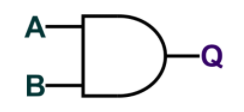
\includegraphics[width=0.2\textwidth]{andGate.PNG}
\begin{table}[H]
    \centering
    \begin{tabularx}{0.127\textwidth}{c|c|c}
    B & A & Q \\
    \hline
    0 & 0 & 0 \\
    0 & 1 & 0 \\
    1 & 0 & 0 \\
    1 & 1 & 1
    \end{tabularx}
    \caption{Truth Table for AND Gate}
\end{table}
Boolean Expression: $Q=A \cdot B$
\subsection{OR Gate}
This outputs 1 when either or both are logic high.
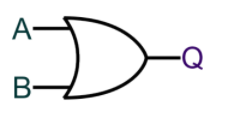
\includegraphics[width=0.2\textwidth]{orGate.PNG}
\begin{table}[H]
    \centering
    \begin{tabularx}{0.127\textwidth}{c|c|c}
    B & A & Q \\
    \hline
    0 & 0 & 0 \\
    0 & 1 & 1 \\
    1 & 0 & 1 \\
    1 & 1 & 1
    \end{tabularx}
    \caption{Truth Table for OR Gate}
\end{table}
Boolean Expression: $Q=A+B$
\subsection{NOT Gate}
This is a single input gate. It inverts the signal in.\\

\includegraphics[width=0.2\textwidth]{notGate.PNG}
\begin{table}[H]
    \centering
    \begin{tabularx}{0.085\textwidth}{c|c}
    A & Q \\
    \hline
    0 & 1 \\
    1 & 0 \\
    \end{tabularx}
    \caption{Truth Table for NOT Gate}
\end{table}
Boolean Expression: $Q=\overline{A}$
\subsection{XOR Gate}
This outputs only when input A or B is logic high - eXclusiveOR.\\
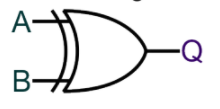
\includegraphics[width=0.2\textwidth]{xorGate.PNG}\\
\begin{table}[H]
    \centering
    \begin{tabularx}{0.127\textwidth}{c|c|c}
    B & A & Q \\
    \hline
    0 & 0 & 0 \\
    0 & 1 & 1 \\
    1 & 0 & 1 \\
    1 & 1 & 0
    \end{tabularx}
    \caption{Truth Table for XOR Gate}
\end{table}
Boolean Expression: $Q = A \oplus B $
\subsection{NAND Gate}
This is the same as an AND gate, except it inverts the output.\\
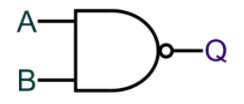
\includegraphics[width=0.2\textwidth]{nandGate.PNG}\\
\begin{table}[H]
    \centering
    \begin{tabularx}{0.127\textwidth}{c|c|c}
    B & A & Q \\
    \hline
    0 & 0 & 1 \\
    0 & 1 & 1 \\
    1 & 0 & 1 \\
    1 & 1 & 0
    \end{tabularx}
    \caption{Truth Table for NAND Gate}
\end{table}
Boolean Expression: $Q = \overline{A \cdot B}$
\subsection{NOR Gate}
This only outputs logic high if both inputs are logic 0 - NotOR. This makes it useful for checking if something is 0.\\
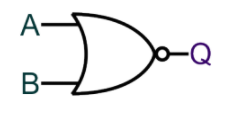
\includegraphics[width=0.2\textwidth]{norGate.PNG}\\
\begin{table}[H]
    \centering
    \begin{tabularx}{0.127\textwidth}{c|c|c}
    B & A & Q \\
    \hline
    0 & 0 & 1 \\
    0 & 1 & 0 \\
    1 & 0 & 0 \\
    1 & 1 & 0
    \end{tabularx}
    \caption{Truth Table for NOR Gate}
\end{table}
Boolean Expression: $Q=\overline{A + B}$
\subsection{XNOR Gate}
This outputs if all inputs are logic 0 or if all inputs are logic 1 - eXclusiveNotOR. This is useful for checking if the inputs are the same.\\
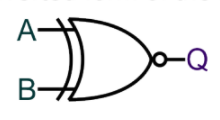
\includegraphics[width=0.2\textwidth]{xnorGate.PNG}\\
\begin{table}[H]
    \centering
    \begin{tabularx}{0.127\textwidth}{c|c|c}
    B & A & Q \\
    \hline
    0 & 0 & 1 \\
    0 & 1 & 0 \\
    1 & 0 & 0 \\
    1 & 1 & 1
    \end{tabularx}
    \caption{Truth Table for XNOR Gate}
\end{table}
Boolean Expression: $Q=\overline{A \oplus B}$

\section{Manually Simplifying Boolean Algebra}
\subsection{Boolean Identities}
$A\oplus B = A \cdot \overline{B} + \overline{A} \cdot B$\\
$\overline{A\oplus B} = A\cdot B + \overline{A} \cdot \overline{B}$
\subsection{Single Variable Rules}
\begin{align*}
    A \cdot 0 &= 0\\
    A \cdot 1 &= A\\
    A \cdot A &= A\\
    A \cdot \overline{A} &= 0\\
    A + 0 &= A\\
    A + 1 &= 1\\
    A + A &= A\\
    A + \overline{A} &= 1
\end{align*}
\subsection{Rules}
\subsubsection{Commutative}
The order doesn't matter.\\
\begin{align*}
    A \cdot B &= B \cdot A\\
    A + B &= B + A
\end{align*}
\subsubsection{Associative}
Some can be re-grouped to make simplification easier.\\
\begin{align*}
    A+(B+C) &= (A+B)+C\\
    &= A+B+C\\ \\
    A\cdot (B\cdot C) &= (A\cdot B) \cdot C \\
    &= A \cdot B \cdot C
\end{align*}
\subsubsection{Distributive}
\begin{align*}
    A\cdot B + A\cdot C &= A(B+C)\\
    C\cdot (B\cdot A + D) &= C\cdot B\cdot A + C \cdot D\\
    (A\cdot B)\cdot (C\cdot D) &= A\cdot C + A\cdot D + \\
    & \ \ \ \ B\cdot C + B\cdot D\\
    A+(B\cdot C) &= (A+B)\cdot (A+C)
\end{align*}
\subsubsection{Absorption / Redundancy}
\begin{align*}
    A+A \cdot B &= A\\
    A+\overline{A} \cdot B &= A+B
\end{align*}
\subsubsection{Double Inversion}
\begin{align*}
    \overline{\overline{A}} &=A
\end{align*}
\subsection{deMorgan's Theorem}
\textit{Break the bar, change the sign}.
\begin{align*}
    \overline{A\cdot B} &= \overline{A} + \overline{B}\\
    \overline{A+B} &= \overline{A}\cdot \overline{B}
\end{align*}

\section{Karnaugh Maps}
Karnaugh maps can be used to simplify boolean algebra expressions. In their simplest form, they have a grid of two across and two down. This is the size which would be needed to simplify a boolean expression for a single logic gate.\\
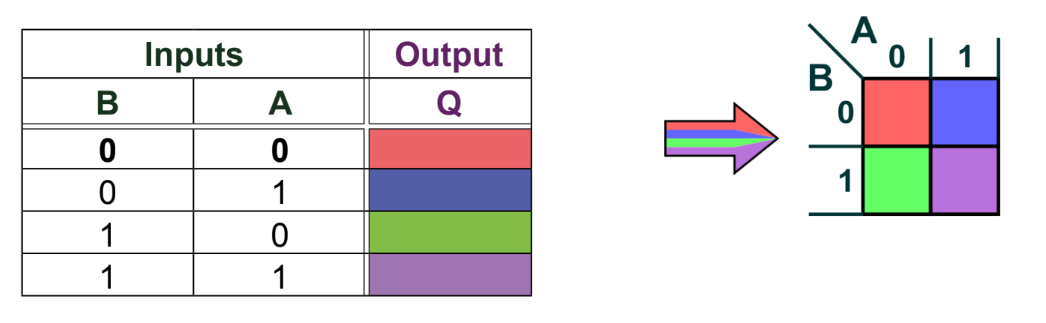
\includegraphics[width=0.45\textwidth]{kMaps1.PNG}\\
\subsection{Simplification using a Karnaugh Map}
Karnaugh maps allow us to simplify boolean expressions graphically. This works by identifying groups of 2, 4 or 8 neighbouring cells containing logic 1 (these can also wrap around the edge of the table); finding the term common to each groups then combining the terms together using the OR operator. Every cell containing logic 1 must be included in at least one group.
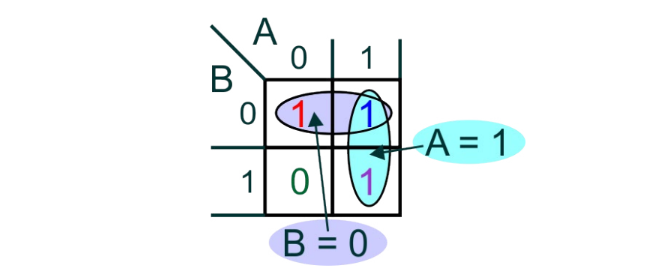
\includegraphics[width=0.45\textwidth]{kMaps2.PNG}\\
In the example above, the top right cell is in two groups, this is okay as long as each group as at least one of the cells in the group is only in one group. The cells in the blue group are in the A=1 column, this means the term common to them is $A$. The cells in the purple group are in the B=0 row, this means the term common to them is $\overline{B}$. Combining the blue and purple group gives us $Q=\overline{B} + A$.
\subsection{Bigger Karnaugh Maps}
Karnaugh maps can have many more inputs. Shown below are three-input and four-input Karnaugh maps.\\
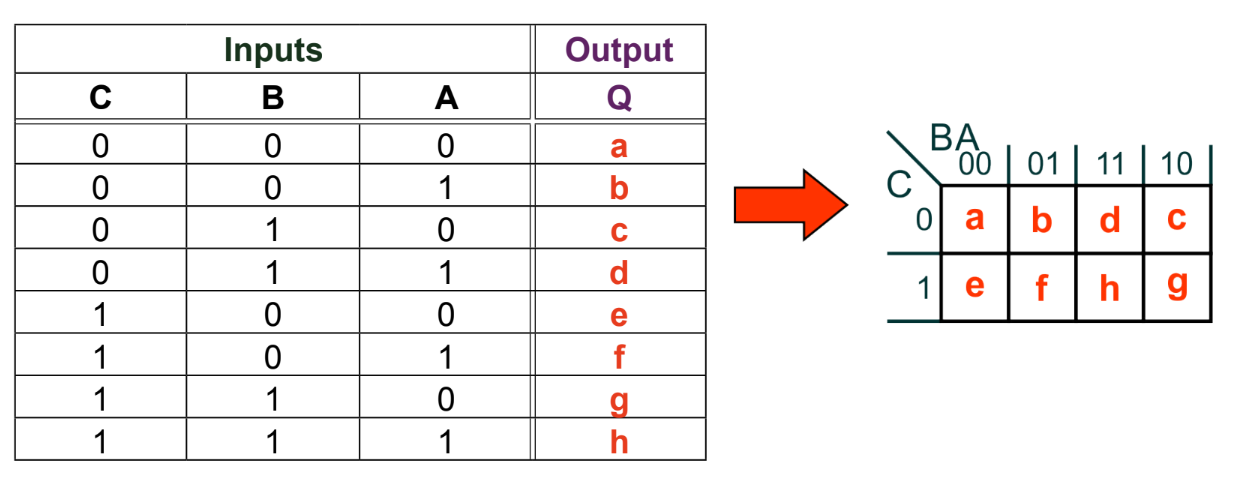
\includegraphics[width=0.45\textwidth]{kMaps CBA inp.PNG}\\
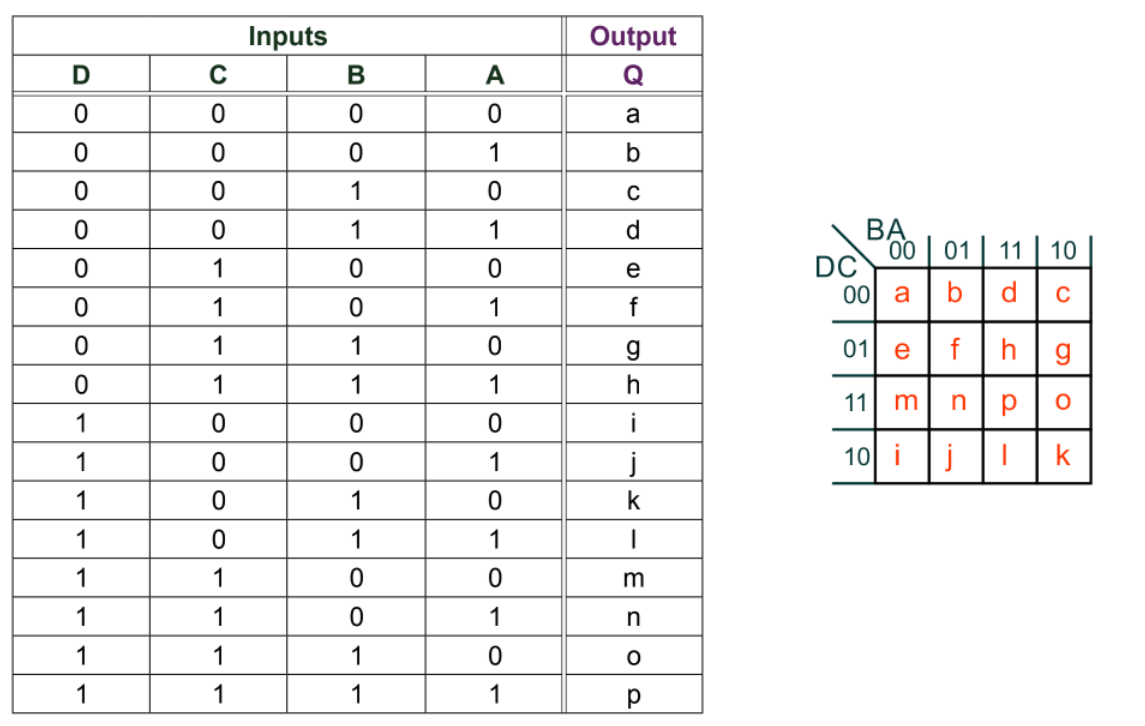
\includegraphics[width=0.45\textwidth]{kMaps DCBA inp.PNG}\\

\section{NAND Gate Conversion}
Any logic gate can be constructed from NAND Gates. This is good as it means the number of chips needed for a circuit can be reduced as you would only need NAND gates. 
The example below shows the stages to go through to convert a system which uses lots of different logic gates into a NAND Gate simplified system.\\
This is the logic system which is going to be converted:\\
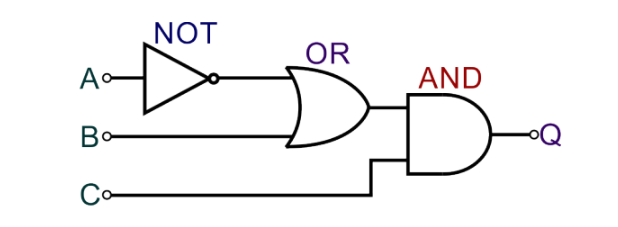
\includegraphics[width=0.45\textwidth]{nand input.PNG}\\
\begin{enumerate}
    \item Replace each gate with its NAND equivalent.
    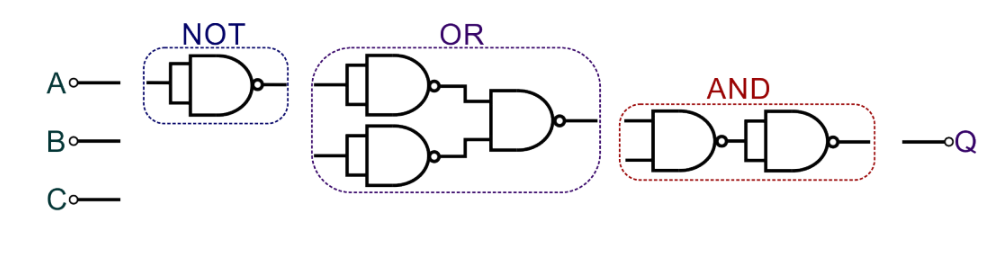
\includegraphics[width=0.4\textwidth]{nand s1.PNG}\\
    \item Connect the equivalents together
    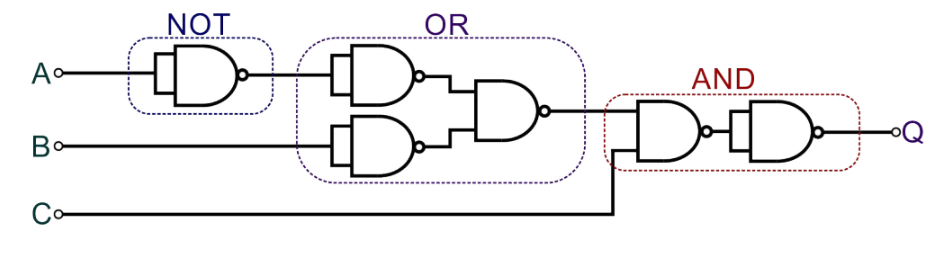
\includegraphics[width=0.4\textwidth]{nand s2.PNG}\\
    \item Cross out redundant gates (gates where there are two single inputs in a row).
    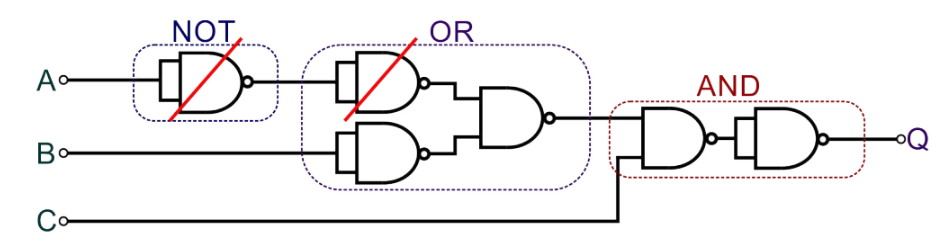
\includegraphics[width=0.4\textwidth]{nand double.PNG}\\
\end{enumerate}
The final circuit is shown below:
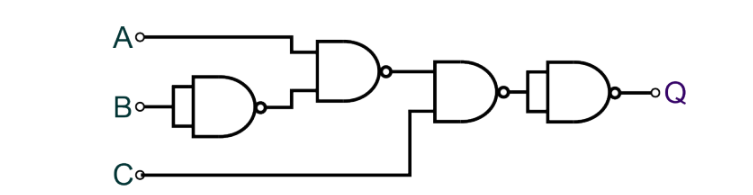
\includegraphics[width=0.45\textwidth]{nand final.PNG}

\section{Multiplexers}
Multiplexers have several inputs and one output. You can select which input is sent to the output. \\
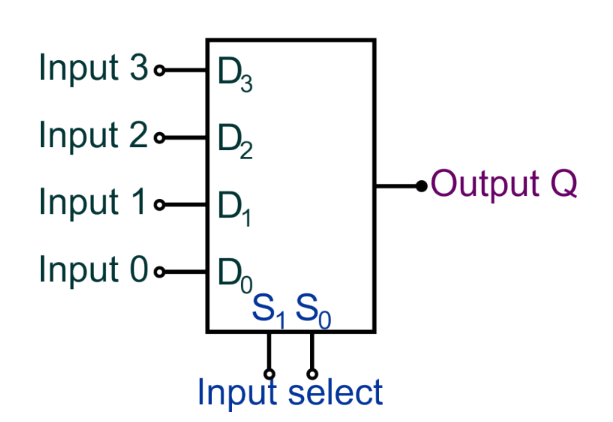
\includegraphics[width=0.3\textwidth]{4-1 mux.PNG}\\
Multiplexers are connected to logic 1 and 0 as shown below:\\
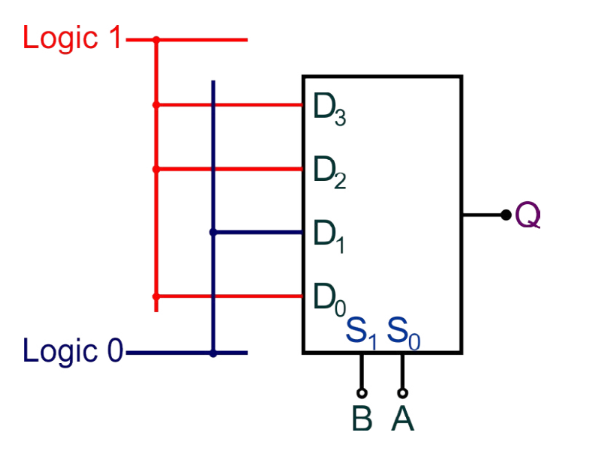
\includegraphics[width=0.3\textwidth]{mux wired.PNG}\\
Multiplexers are useful for complicated logic systems where a large number of logic gates would otherwise be required. 


\end{document}
